\documentclass[a4paper]{article}

\usepackage{lmodern}

%% Language and font encodings
\usepackage[french]{babel}
\usepackage[utf8x]{inputenc}
\usepackage[T1]{fontenc}
\usepackage{enumitem}
\usepackage{xcolor}
\usepackage{pifont}

%% Sets page size and margins
\usepackage[a4paper,top=3cm,bottom=3cm,left=2cm,right=2cm,marginparwidth=2cm]{geometry}
%% Useful packages
\usepackage{amsmath}
\usepackage{graphicx}
\usepackage[colorinlistoftodos]{todonotes}
\usepackage[colorlinks=true, allcolors=black]{hyperref}
\usepackage{fourier-orns}
\usepackage{titlesec}
\usepackage{fancyhdr}
\usepackage{fancyvrb}
%\renewcommand{\thefootnote}{\*}
\pagestyle{fancy} 
\setcounter{tocdepth}{5}
\usepackage{array}



%% Tikz stuff
\usepackage{tikz}
\usetikzlibrary{calc, arrows}
\tikzstyle{incolore} = [rectangle, rounded corners, draw=black, minimum height=1cm, minimum width=3cm, text width=3cm, text centered]
\usepackage{float}

\usepackage{makecell}
\usepackage{libertine}
\newcommand{\hsp}{\hspace{20pt}}
\newcommand{\HRule}{\rule{\linewidth}{0.5mm}}





\renewcommand{\headrulewidth}{1pt}
\fancyhead[C]{} 
\fancyhead[L]{}
\fancyhead[R]{\footnotesize{\leftmark}}

\renewcommand{\footrulewidth}{1pt}
\fancyfoot[C]{} 
\fancyhead[L]{}
\fancyfoot[R]{\thepage}

\definecolor{Zgris}{rgb}{0.87,0.85,0.85}

\usepackage{eso-pic,graphicx}
\usepackage{xcolor}
\newcommand{\bgimg}[1]{
\AddToShipoutPicture
   {
      \put(\LenToUnit{0 cm},\LenToUnit{0 cm})
      {
            \includegraphics[width=\paperwidth,height=\paperheight]{#1} 
      }
   }
}


\begin{document}


%%\bgimg{Image_15.jpg}





  \begin{titlepage}
    \begin{sffamily}
    \begin{center}
      \textnormal{}\\[6.5cm]
      % Upper part of the page. The '~' is needed because \\
      % only works if a paragraph has started.
      % Title
      \HRule \\[0.4cm]
      { \Huge \bfseries Synthèse\\ Principe de sécurité informatique\\ [0.4cm] }
      \HRule \\[3cm]
      \Large
      Deuxième Bloc\\
      Sécurité des systèmes\\
      Année académique 2020-2021\\[0.2cm]
      \emph{Rédigé par Sénéchal Julien}
      \vfill
      % Bottom of the page
      {\large 23 Décembre 2020}
    \end{center}
    \end{sffamily}
  \end{titlepage}

  \section{Liste des actions à entreprendre suite à la découverte d'un RansomWare}
  \begin{enumerate}
    \item Ouvrir une main courante (toute action doit y être noté)
    \item Isoler tous les équipements infectés du réseau
    \item Déconnecter les entrées possibles de l'attaquant pour limiter l'attaque en cours (Donc surtout Internet)
    \item Appeler à l'aide les services prévu à cet effet :
    \begin{itemize}[label=\ding{228}, font=\scriptsize]
      \item Police, CERT.BE
      \item Prestataire spécialisé (il est mieux de l'avoir choisi en amont)
      \item Une éventuelle Assurance
    \end{itemize}
    \item Assurer la communication avec :
    \begin{itemize}[label=\ding{228}, font=\scriptsize]
      \item La hiérarchie
      \item le métier
      \item l'extérieur
    \end{itemize}
    \item Lancer le plan de continuité des services (redondance, pasage en mode dégradé si possible)
    \item Si des données à caractères personnel ont été touché, prévenir l'Autorité de Protection des données (APD.be) (Attention au délai légal)
    \item Trouver le programme malveillant (ex : Vérifier les logs)
    \item Supprimer le RansomWares du système informatique infecté
    \item Réinstaller l'OS si nécessaire (dans une version à jour)
    \item Corriger les vulnérabilités du point d'entrée de l'attaquant
    \item Restaurer les données grâce a un back-up sain
  \end{enumerate}

  \section{Les ransomwares}
  \begin{itemize}[label=\textbullet, font=\Large]
    \item Big Game Huntig
    \begin{itemize}[label=\ding{228}, font=\scriptsize]
      \item Attaques par ransomwares qui portent sur des victimes au moyens financiers importants. (trad : La chasse au gros)
    \end{itemize}
    \item Attaque indirecte
    \begin{itemize}[label=\ding{228}, font=\scriptsize]
      \item Cibler des entreprises sous-traitantes ou clé du secteur dans le but de déstabiliser le secteur ce qui engendre un impact que le secteur.
      \item Conséquences :
      \begin{itemize}
        \item Arrêt de production
        \item Chute du chiffre d'affaire
        \item Risques judiciaire (RGPD)
        \item Réputation
        \item Perte de confiance des clients
        \item Rupture ou dégradation de l'activité chez la victime donc impoacts sur ceux qui sont liés à l'activité
      \end{itemize}
    \end{itemize}
    \item Payer la rançon ?
    \begin{itemize}[label=\ding{228}, font=\scriptsize]
      \item Auncune garantie de récupérer ses données
      \item Si ça fonctionne, ça retarde le problème et ne grantit pas la protection contre une seconde attaque
    \end{itemize}
    \item Comment réduire les pertes en cas d'attaque par ransomware ?
    \begin{itemize}[label=\ding{228}, font=\scriptsize]
      \item Backup régulier (idéalement hors-ligne)
      \item Maintien en condition de la sécurité par des correctifs
      \item Mise à jour des signatures antivirus
      \item Mettre en oeuvre une politique de filtrage sur les postes de travail
      \item Désactiver les droits administrateur pour les utilisateurs
      \item Segmentation du réseau
      \item Limitation des privilèges accordés aux utilisateurs
      \item Maîtrise des accès a internet
      \item Sensibilisation aux risques
    \end{itemize}
    \item 2 axes techniques pour s'en défendre
    \begin{itemize}[label=\ding{228}, font=\scriptsize]
      \item sécurité des réseaux (segmentation, limitation des privilèges)
      \item sécurité des OS
    \end{itemize}
    \item Besoin d'un backup même si des snapchots de machine virtuelles sont stockés sur un SAN ou NAS (Backup-less)
    \begin{itemize}[label=\ding{228}, font=\scriptsize]
      \item L'usage de solutions de stockage à froid permet de protéger les sauvegardes d'une infection des systèmes et de conserver 
      les données critiques à la reprise d'activité
      \item Conseillé de garder ses données à plusieurs endroits et de les maintenir à jour
    \end{itemize}
    \item Si on ne peut pas patcher un poste, on doit prendre des mesures d'isolement
    \item Rôle des CERT dans la lutte contre les ransomwares
    \begin{itemize}[label=\ding{228}, font=\scriptsize]
      \item Assurent une veille permanente qui permet de rester informé de la découverte (des failles, type d'attaque, etc...)
      \item Donnent des conseils en cas d'accident
      \item Observent et analysent les problèmes de sécu en ligne et en informe l'audience
    \end{itemize}
    \item Fonctions assurées par une passerelle Internet sécurisé
    \begin{itemize}[label=\ding{228}, font=\scriptsize]
      \item Filtrer les tentatives de connexion en fonction de la catégorisation ou de la réputation des sites que vos collaborateurs tentent de visiter
      \item Identifier les activités anormales
    \end{itemize}
    \item Problème de la journalisation
    \begin{itemize}[label=\ding{228}, font=\scriptsize]
      \item Se fait en temps réel, donc difficile de tout vérifier et de s'en rendre compte au moment opportun
      \item Son but est de permettre de découvrir un problème mais pas de le prévenir
    \end{itemize}
    \item Rôle d'un plan de continuité
    \begin{itemize}[label=\ding{228}, font=\scriptsize]
      \item Permet de fonctionner quand survient une altération plus ou moins sévère du système d'information
    \end{itemize}
    \item Personnes concerné par un exercice de prévention :
    \begin{itemize}[label=\ding{228}, font=\scriptsize]
      \item TOUT LE MONDE doit savoir protéger ses informations
    \end{itemize}
    \item Contenu d'une main courant
    \begin{itemize}[label=\ding{228}, font=\scriptsize]
      \item heure, date, action
      \item nom de la personne qui fait l'action
      \item description de l'action
    \end{itemize}
    \item RETEX
    \begin{itemize}[label=\ding{228}, font=\scriptsize]
      \item Retour d'expérience
    \end{itemize}
    \item Porter plainte contre X au CERT et à la police lors d'une attaque par RansomWare
    \item No More Ransom
    \begin{itemize}[label=\ding{228}, font=\scriptsize]
      \item Recensement des moyens de déchiffrement applicables à un grand nombre de rançonlogiciels
    \end{itemize}
  \end{itemize}

\section{Quick-Wins}
\begin{enumerate}
  \item Supervisez les antivirus
  \item Migrez les administrateurs dans Protected Users
  \item Scannez votre espace d'adresses IP 
  \item Développez la connaissance des applications et leurs propriétaires
  \item Activez le multi-facteur dans le cloud
  \item Supprimez \emph{seDebugPrivilege} (privilège permettant de lire la mémoire de n'importe quel processus)
  \item Identifiez les prestataires DFIR (digital forensics \& incident response)
  \item Déployez un outil de gestion de mot de passe
  \item Utilisez HaveIBeenPowned
  \item Bloquez les IP suspectes sur les services exposés
\end{enumerate}

\section{Questions sur les Quick-Wins}
\begin{itemize}[label=\textbullet, font=\Large]
  \item Le groupe Windows Protected Users est-il utilisable dans une foret AD hétérogène ?
  \begin{itemize}[label=\ding{228}, font=\scriptsize]
    \item Non si l'OS est trop vieux car cette fonctionnaité n'existe que depuis la version Windows Server 2012. Pour les serveurs plus vieux, il faut une forêt dédié
  \end{itemize}
  \item Quel outil peut être utilisé pour vous aider à scanner votre espace d'adresses IP ?
  \begin{itemize}[label=\ding{228}, font=\scriptsize]
    \item nmap (scan de port)
  \end{itemize}
  \item Qu'est-ce que le propriétaire d'une application dans un contexte professionnel d'entreprise ? (business owner)
  \begin{itemize}[label=\ding{228}, font=\scriptsize]
    \item Personne responsable de l'application
  \end{itemize}
  \item  L'activation d'un second facteur d'authentification, même si ce dernier n'est pas techniquement parfait, ce sera toujours mieux qu'un seul facteur d'authentification ?
  \begin{itemize}[label=\ding{228}, font=\scriptsize]
    \item Vrai car toujours plus de travail pour attaquer le système et peur donc démotiver le hacker. Ca peut aussi être utilisé le temps d'en trouver un meilleur
  \end{itemize}
  \item Connaître le nom des "pompiers" de l'informatique en cas "d'incendie" pour ainsi dire (prestataire DFIR - figital forensics \& incident response)
  \begin{itemize}[label=\ding{228}, font=\scriptsize]
    \item Nviso
    \item PWC
    \item KPGM
    \item Deloitee
    \item Ernst \& Young
  \end{itemize}
  \item Gestionnaire de mot de passe open source
  \begin{itemize}[label=\ding{228}, font=\scriptsize]
    \item KeePass
    \item BitWarden
  \end{itemize}
  \item Utilité de HaveIBeenPowned
  \begin{itemize}[label=\ding{228}, font=\scriptsize]
    \item Savoir si des informations liées à votre adresse mail ont fuité (mot de passe, nom, etc..)
  \end{itemize}
\end{itemize}

\section{CVE-CVSS}
\textbf{Ce chapitre est exclusivement le travail de Florian Nicolas, merci à lui !}
\begin{itemize}[label=\textbullet, font=\Large]
  \item Définition
  \begin{itemize}[label=\ding{228}, font=\scriptsize]
    \item C’est un système de score permettant de mesurer l’exposition au danger d’une vulnérabilité
  \end{itemize}
  \item CVSS utilise trois groupe de métriques pour évaluer une vulnérabilité :
  \begin{itemize}[label=\ding{228}, font=\scriptsize]
    \item Groupe de métrique de base
    \begin{itemize}
      \item Représente les caractèristiques d'une vulnérabilité qui est invariable dans le temps
    \end{itemize}
    \item Groupe de métrique temporaire
    \begin{itemize}
      \item Mesure les caractèristiques de la vulnérabilité qui peut changer mais pas en dehors de l'environnement de l'utilisateur
    \end{itemize}
    \item Groupe de métrique environnementale
    \begin{itemize}
      \item Mesure les aspect de la vulnérabilité qui sont spécifiques à l'environnement de l'organisation
      \begin{figure}[H]
        \centering
        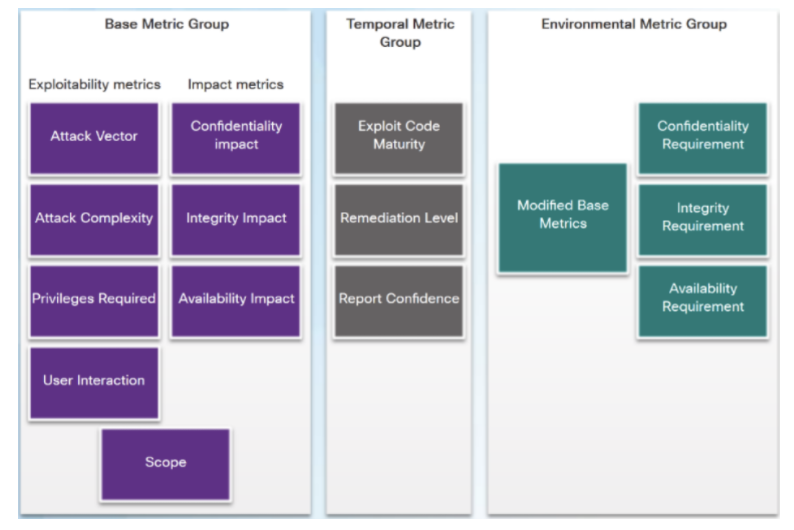
\includegraphics[width=12cm]{images/CVSS.PNG}
        \caption{Groupes Métriques}
        \end{figure}
    \end{itemize}
  \end{itemize}
  \item CVSS Base metric group
  \begin{itemize}[label=\ding{228}, font=\scriptsize]
    \item Inclus
    \begin{itemize}
      \item Vecteur d'attaque
      \item Complexité de l'attaque
      \item Privilèges requis
      \item Interaction de l'utilisateur
      \item Objectif
    \end{itemize}
    \item Inclus les impacts sur :
    \begin{itemize}
      \item la confidentialité
      \item l'intégrité
      \item la disponibilité
    \end{itemize}
  \end{itemize}
  \item CVSS v3.0 calculator
  \begin{itemize}[label=\ding{228}, font=\scriptsize]
    \item Similaire à un questionnaire où chaque choix sont faits pour décrire la vulnérabilité rencontrée pour un groupe métrique
    \item Le score de la vulnérabilité sera généré
  \end{itemize}
  \item CVSS reports
  \begin{itemize}[label=\ding{228}, font=\scriptsize]
    \item Manière dont une vulnérabilité est mesurée :
    \begin{figure}[H]
      \centering
      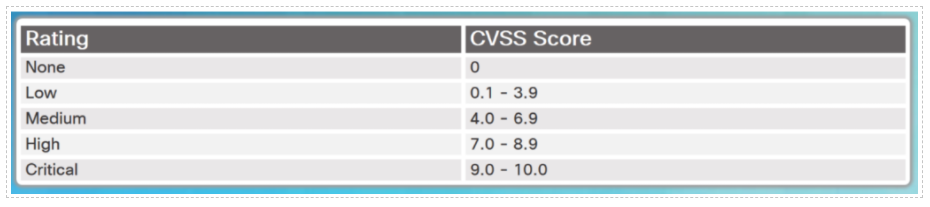
\includegraphics[width=17cm]{images/reports.PNG}
      \caption{Groupes Métriques}
      \end{figure}
  \end{itemize}
\end{itemize}

\section{Place de la sécurité dans l'entreprise}
\begin{itemize}[label=\textbullet, font=\Large]
  \item Une entreprise définit son identité par des \textbf{valeurs}
  \begin{itemize}[label=\ding{228}, font=\scriptsize]
    \item Exemples : Innovation, qualité, intégrité, satisfaction client, etc... (Mots à choisir avec soin)
  \end{itemize}
  \item Les valeurs permettent de définir la \textbf{mission} et la \textbf{vision} de l'entreprise
  \begin{itemize}[label=\ding{228}, font=\scriptsize]
    \item Mission : définition de sa raison d'être
    \item Vision : l'état futur désiré
  \end{itemize}
  \item La mission et la vision se déclienent en \textbf{stratégie(s)}
  \begin{itemize}[label=\ding{228}, font=\scriptsize]
    \item Stratégie : La détermination des orientations à long terme de l'entreprise et l'adoption des actions y compris 
    l'allocation des ressources nécessaire à la réalisation de ces objectifs
  \end{itemize}
  \item La/Les stratégie(s) se concrétise en \textbf{politique(s)}
  \begin{itemize}[label=\ding{228}, font=\scriptsize]
    \item Nécessite
    \begin{itemize}
      \item de former pour utiliser cette politique
      \item de sensibiliser le personnel
    \end{itemize}
    \item Caractéristiques
    \begin{itemize}
      \item Simple et compréhensible
      \item Facilement réalisable
      \item Vérifiable et contrôlable
      \item Durée de vie : 3-4 ans
    \end{itemize}
  \end{itemize}
  \item Une des stratégie de l'entreprise est la stratégie de sécurité de l'information
  \item Découle de cette stratégie la \textbf{polittique de securite informatique}
  \begin{itemize}[label=\ding{228}, font=\scriptsize]
    \item Déclinable en plusieurs documents
    \begin{itemize}
      \item Politique de contrôle d’accès
      \item Politique de gestion des droits numériques
      \item Politique de prévention
      \item Politique de protection
      \item etc...
    \end{itemize}
    \item Chaque focument est composé d'une partie sur :
    \begin{itemize}
      \item Les bonnes pratiques
      \item Une analyse des risques + une methodologie dediee
      \item La loi
      \item Une analyse des risques systematiqueent fondee sur les retours d'experience des utilisateurs (Single point of contact)
      \item Toute autre source d'information jugée utile
    \end{itemize}
    \item Chaque document est complété par des procédures et documentations techniques
  \end{itemize}
\end{itemize}



























\end{document}